\subsection{Entwurfsmuster}\label{subsec:entwurfsmuster}


Zu den Voraussetzungen, die von der Testinfrastruktur erwartet werden,
gehört die Hohe Wartbarkeit der Testsuite. Dieses Ziel könnte ohne die
Verwendung von Entwurfsmustern nicht erreicht werden. Entwurfsmuster
können den Entwicklungsprozess beschleunigen, indem sie getestete, bewährte
Entwicklungsparadigmen bereitstellen. Ein effektiver Softwareentwurf
erfordert die Berücksichtigung von Problemen, die möglicherweise erst
später bei der Implementierung sichtbar werden. Die Wiederverwendung von
Entwurfsmustern hilft, subtile Probleme zu vermeiden, die zu großen
Problemen führen können, und verbessert die Lesbarkeit des Codes für
Programmierer und Architekten, die mit den Mustern vertraut sind.  Für die
Entwicklung von Tests mit Selenium gibt es zwei Entwurfsmuster, die sehr
beliebt sind und von Testern verwendet werden :
\textbf{Page Object} und \textbf{Factory} (vgl. \cite{pattern-browser}).

\subsubsection{Page Object Model}

Page Object Model ist ein in Selenium verwendetes Entwurfsmuster,
bei dem ein Objektrepository zur Speicherung von WebElementen
erstellt wird. Es wird eine Java-Klasse erstellt, die jeder WebSeite
entspricht (siehe \Cref{fig:page-obj}). Diese Seiten bestehen aus WebElementen und den
entsprechenden Methoden, die auf diese Elemente einwirken (siehe \Cref{fig:page-exp}).
Alle Webseitenelemente befinden sich in einer Java-Klasse, indem sie durch
ihre Locators identifiziert werden.  Darüber hinaus werden für die
verschiedenen Seiten der Webseite mehrere Java-Klassen erstellt. Diese
Java-Klassen dienen als Repository, in dem die verschiedenen Elemente
gespeichert werden, mit denen Testfällen interagieren können. Die Verwendung
des Page Object Model hat viele Vorteile:

\begin{enumerate}
    \item \textbf{Erleichtert die Wartung des Codes} : Da die Testklassen von den
    Klassen getrennt sind, die die Webelemente und die Operationen auf
    ihnen enthalten, ist die Aktualisierung des Codes sehr einfach, wenn
    ein Webelement aktualisiert oder ein neues hinzugefügt wird.
    \item \textbf{Erleichtert die Lesbarkeit des Codes} : Der Benutzer kann das Projekt
    und die Testskripte aufgrund der feinen Trennung zwischen den Testklassen
    und den verschiedenen Webseiten leicht durchlesen.
    \item \textbf{Wiederverwendbarkeit des Codes} : Wenn mehrere Testskripte dieselben
    Webelemente verwenden, müssen nicht in jedem Testskript Code zur
    Behandlung des Webelements geschrieben werden. Die Unterbringung in einer
    separaten Seitenklasse macht es wiederverwendbar, indem es von jedem
    Testskript aus zugänglich gemacht wird.
\end{enumerate}

\begin{figure}[H]
    \centering
    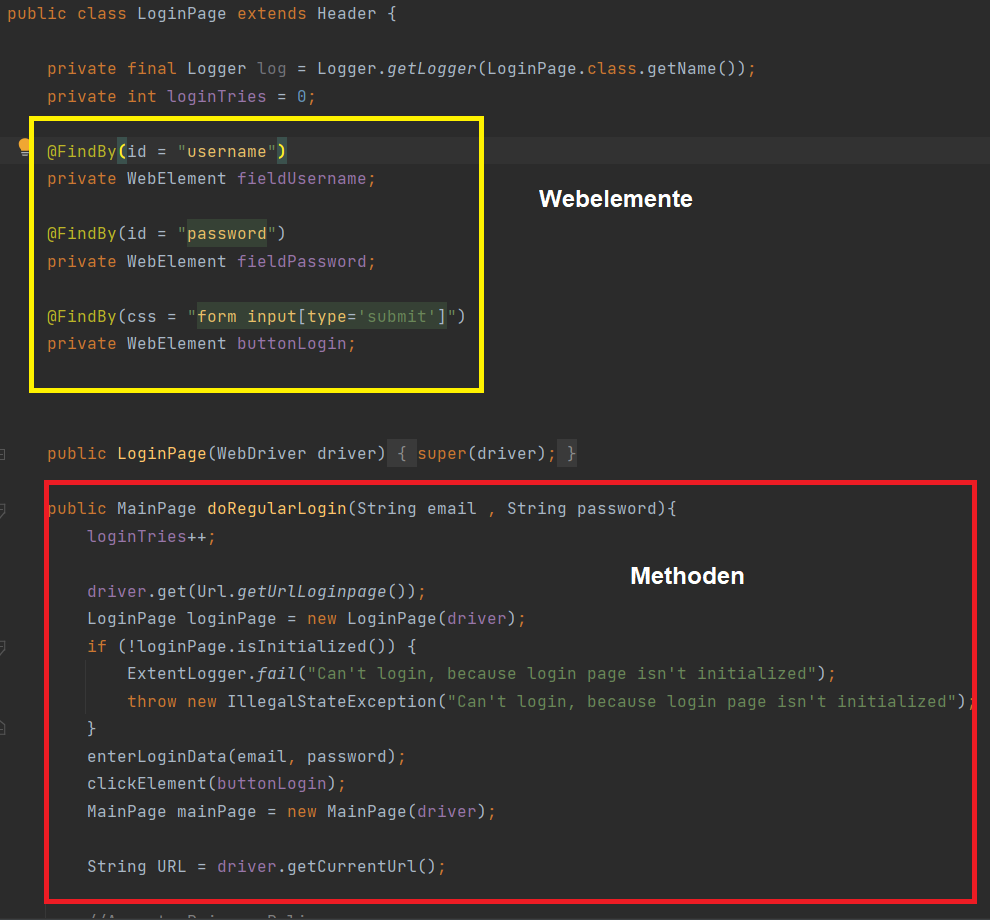
\includegraphics[scale=0.5]{images/page-example}
    \caption{Darstellung der jExam LoginPage mit dem Page Object Model} \label{fig:page-exp}
\end{figure}

\begin{figure}[H]
    \centering
    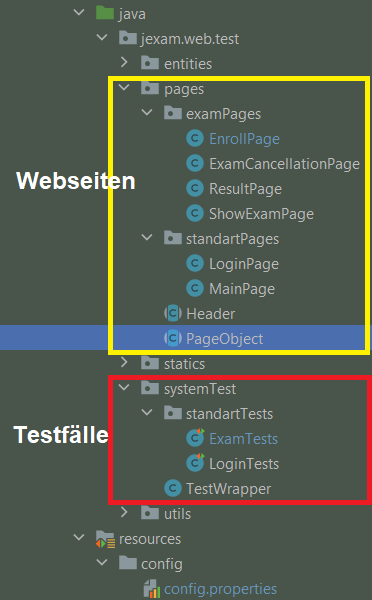
\includegraphics[scale=0.6]{images/page-object}
    \caption{Projektstruktur von jExam Page Object Model} \label{fig:page-obj}
\end{figure}

\subsubsection{Factory}

Page Factory ist eine Klasse, die von Selenium WebDriver bereitgestellt
wird, um das Page Object Model zu implementieren. Das Page Object
Repository wird mit Hilfe des Page Factory-Konzepts von den Testmethoden
getrennt. Page Factory bietet Annotationen, um Elemente zu initialisieren und sie
anschaulich und lesbar macht. Zu den Vorteilen seiner Verwendung gehören:

\begin{enumerate}
    \item \textbf{Sauberer Code}: Das definierte Webelement wird von den Methoden
    getrennt, um eine Webseite in einer Page Object sauber und
    aufgeräumt zu gestalten.
    \item \textbf{Lesbar und beschreibend}: Ein Webelement wird als Variable
    (bekannt als Object Field) deklariert, und die Field-Annotation
    (@FindBy siehe \Cref{fig:page-exp}) wird verwendet, um den Namen, den Typ und
    die Position des Elements zu beschreiben. Auf diese Weise können
    definierte Webelement anhand seiner Annotationen wie Name, Typ
    usw. leicht identifiziert werden.
    \item \textbf{Einfache Wartbarkeit}: Das definierte Webelement kann ohne
    Neudefinition überall in der Page Object Klasse und den Unterklassen
    verwendet werden. Das bedeutet, dass ein bestimmtes Webelement
    mehrmals verwendet werden kann, aber nur an einer Stelle
    definiert ist.
\end{enumerate}


Im nächsten Teil werden die Implementierung der Tests und die verwendeten
Methoden genauer beschrieben.




